\documentclass{article}
\usepackage[spanish]{babel}
\usepackage[utf8]{inputenc}
\usepackage[T1]{fontenc}
\usepackage{hyperref}
\usepackage{xcolor}
\usepackage{listings}
\usepackage{minted}
\usepackage{graphicx}
\hypersetup{
    colorlinks,
    linkcolor={red!50!black},
    citecolor={blue!50!black},
    urlcolor={blue!80!black}
}

\title{P1: Desarrollo de una Web}
\author{Daniel Ramos}
\date{\today}

\begin{document}

\maketitle

\begin{center}
    \large Herramientas HTML y CSS I
\end{center}

\newpage

\tableofcontents

\newpage

\section*{Introducción}

En esta práctica, aprenderemos a configurar el entorno de desarrollo necesario para trabajar con HTML y CSS. Esto incluye la instalación de editores de texto, navegadores web y otras herramientas útiles. Además, se ha desarrollado una página web sencilla para poner en práctica lo aprendido. Este documento detalla los pasos seguidos, las herramientas utilizadas y las configuraciones realizadas, proporcionando una guía completa para replicar el proceso. Para poder llevar a cabo la corrección de la práctica se proporcionan a continuación los enlaces a la página web y al repositorio de Github:

\begin{itemize}
    \item \href{https://github.com/DanielRamosAcosta/hhyc-dramosac}{Repositorio en GitHub}
    \item \href{https://www.danielramos.me/hhyc-dramosac}{Página web desplegada}
\end{itemize}

\newpage

\section{Configurando el Entorno de Desarrollo}\label{sec:configurando-el-entorno-de-desarrollo}

\subsection{Estableciendo la Base del Proyecto}\label{subsec:estableciendo-la-base-del-proyecto}

El primer paso ha sido inicializar el repositorio en el que se hará el desarrollo de la práctica con \mintinline{bash}{git init} y \mintinline{bash}{npm init}. Esto asegura que el proyecto esté correctamente versionado y que se puedan gestionar las dependencias de manera eficiente.

Siguiendo la guía de la web de Parcel, lo siguiente ha sido instalar Parcel como dependencia del proyecto con \mintinline{bash}{npm install --save-dev parcel}. Parcel es una herramienta moderna que simplifica la construcción y el empaquetado de aplicaciones web.

Una vez instalado Parcel, se ha probado su correcto funcionamiento creando un \textit{Hello World}. Para ello, se creó el fichero \mintinline{bash}{src/index.html} y se ejecutó el comando \mintinline{bash}{npx parcel src/index.html}. Esto permitió verificar que la página web se abría correctamente en el navegador, como se muestra en la Figura~\ref{fig:hello-world}.

 \begin{figure}[h!]
     \centering
     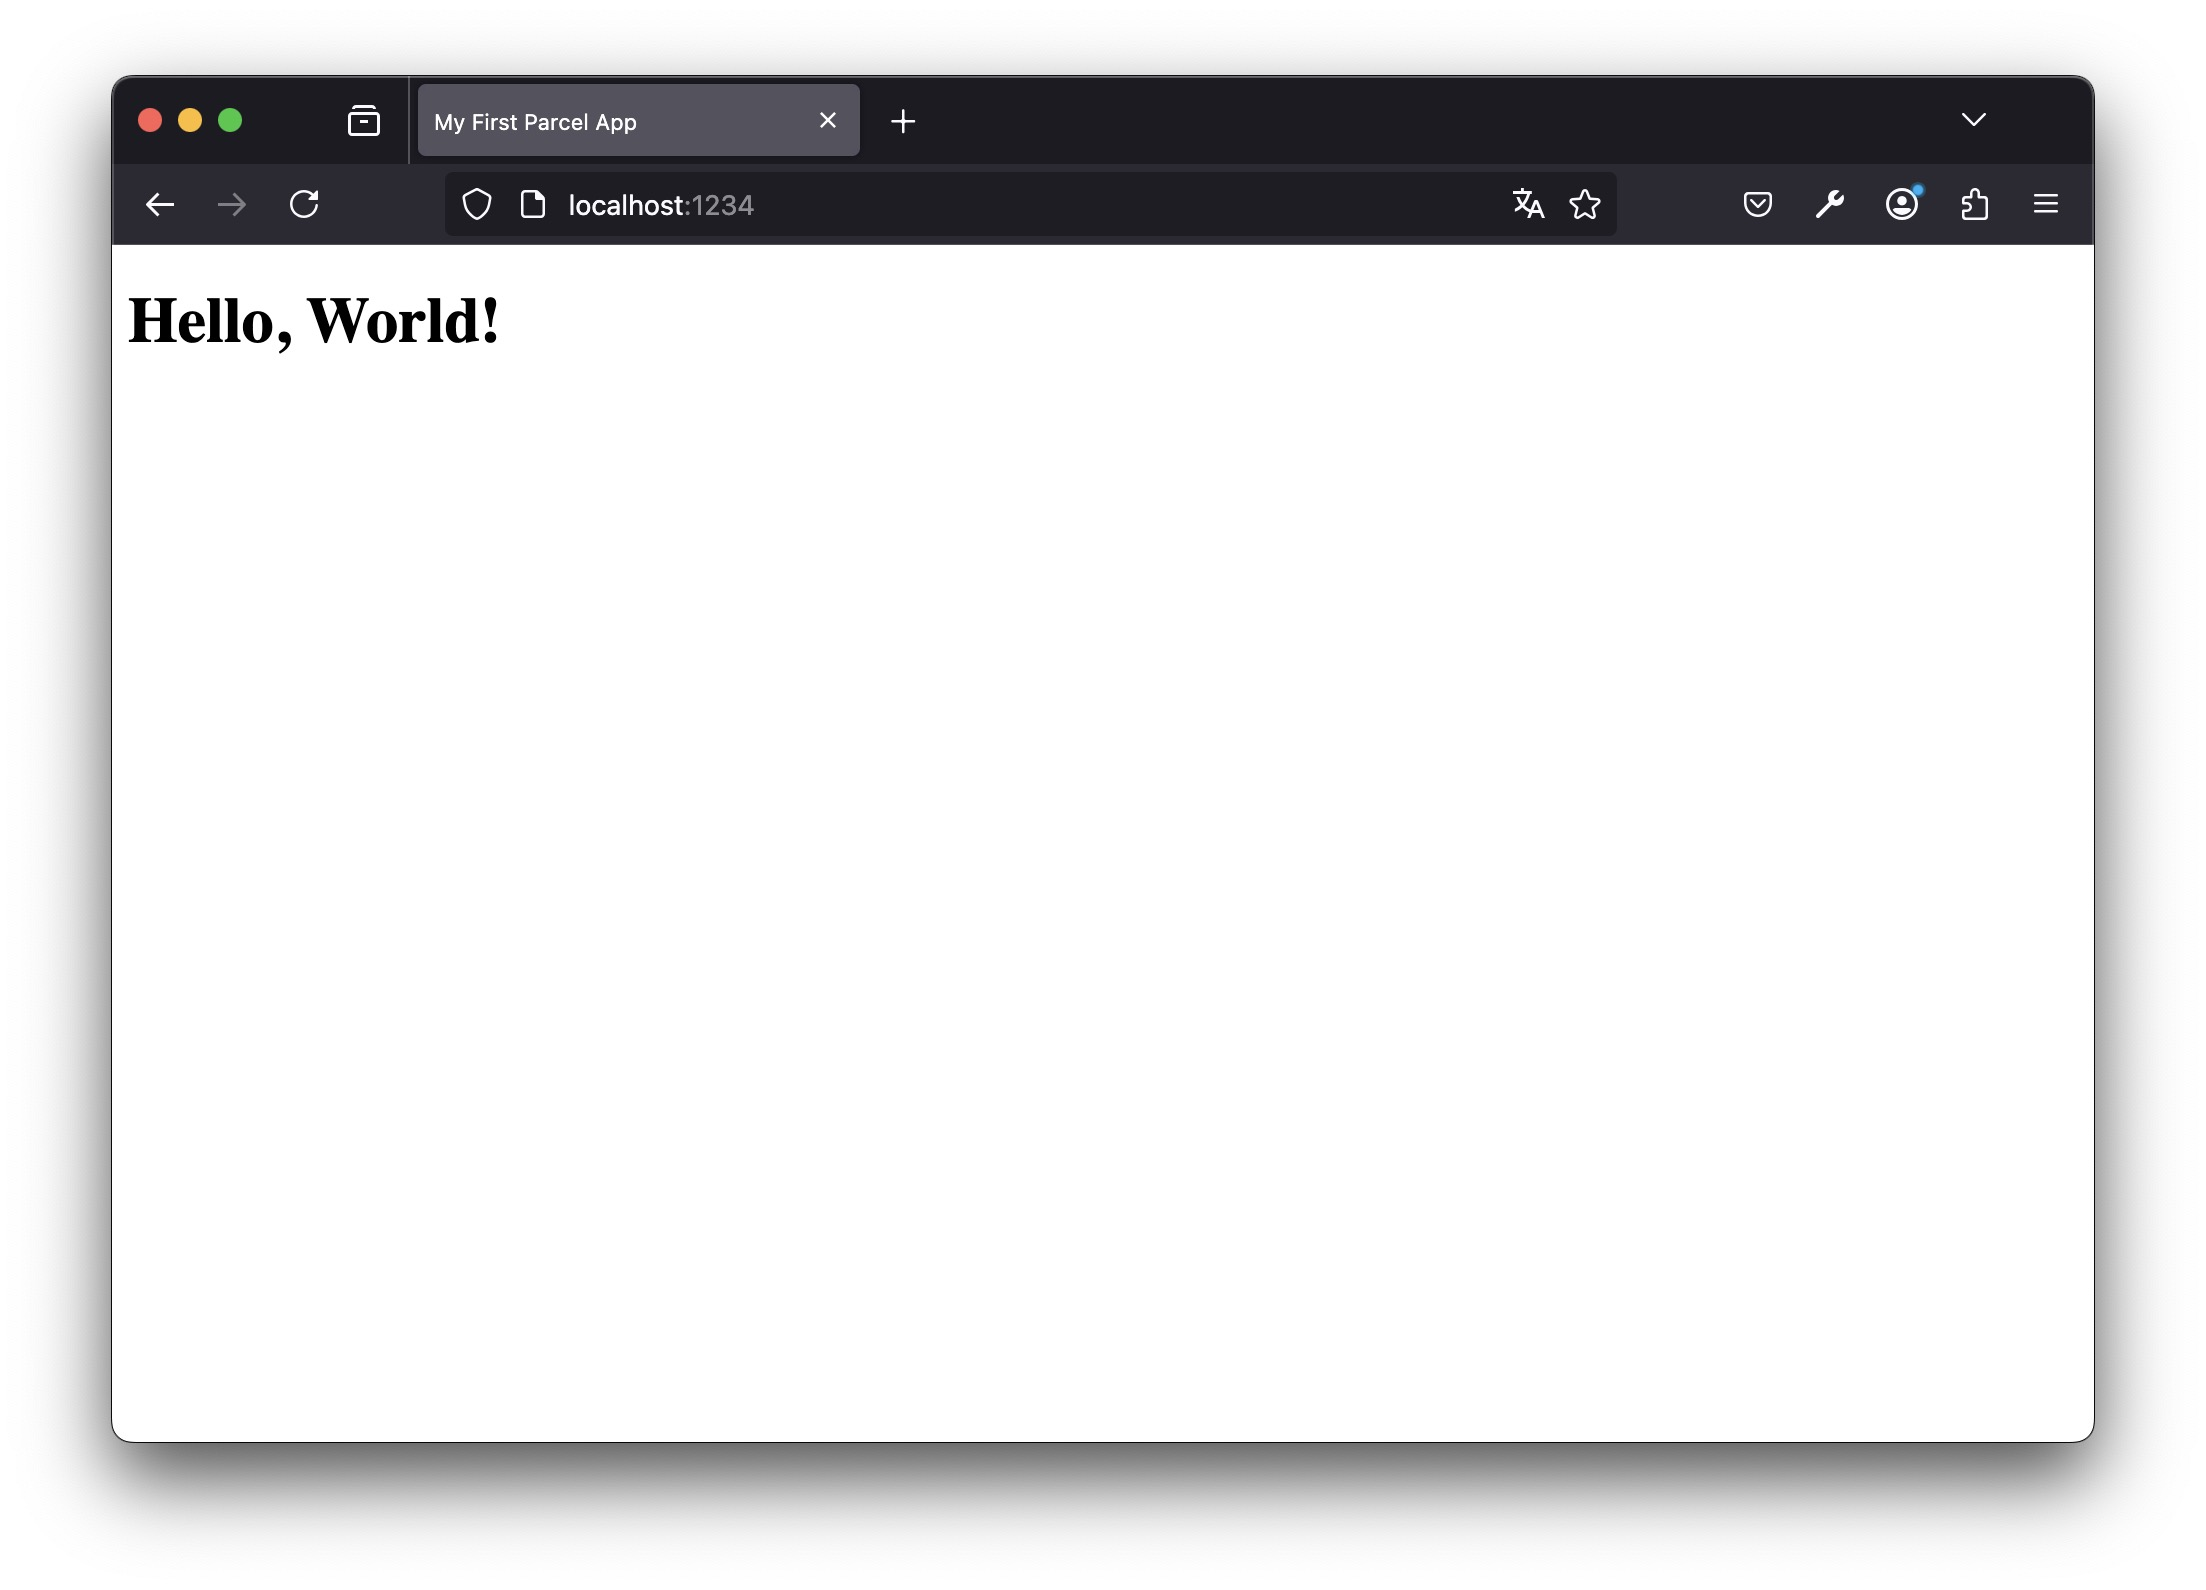
\includegraphics[width=0.8\textwidth]{./img/p1/hello-world}
     \caption{Captura de pantalla de un Hello World básico en HTML}
     \label{fig:hello-world}
 \end{figure}

Se realizaron las modificaciones necesarias para incluir una hoja de estilos y un script de ejemplo, comprobando que Parcel procesaba ambos correctamente. Sin necesidad de refrescar el navegador, los cambios se reflejaron instantáneamente en la página web (ver Figura~\ref{fig:parcel}). Esto demuestra la potencia de Parcel para agilizar el flujo de trabajo.

 \begin{figure}[h!]
     \centering
     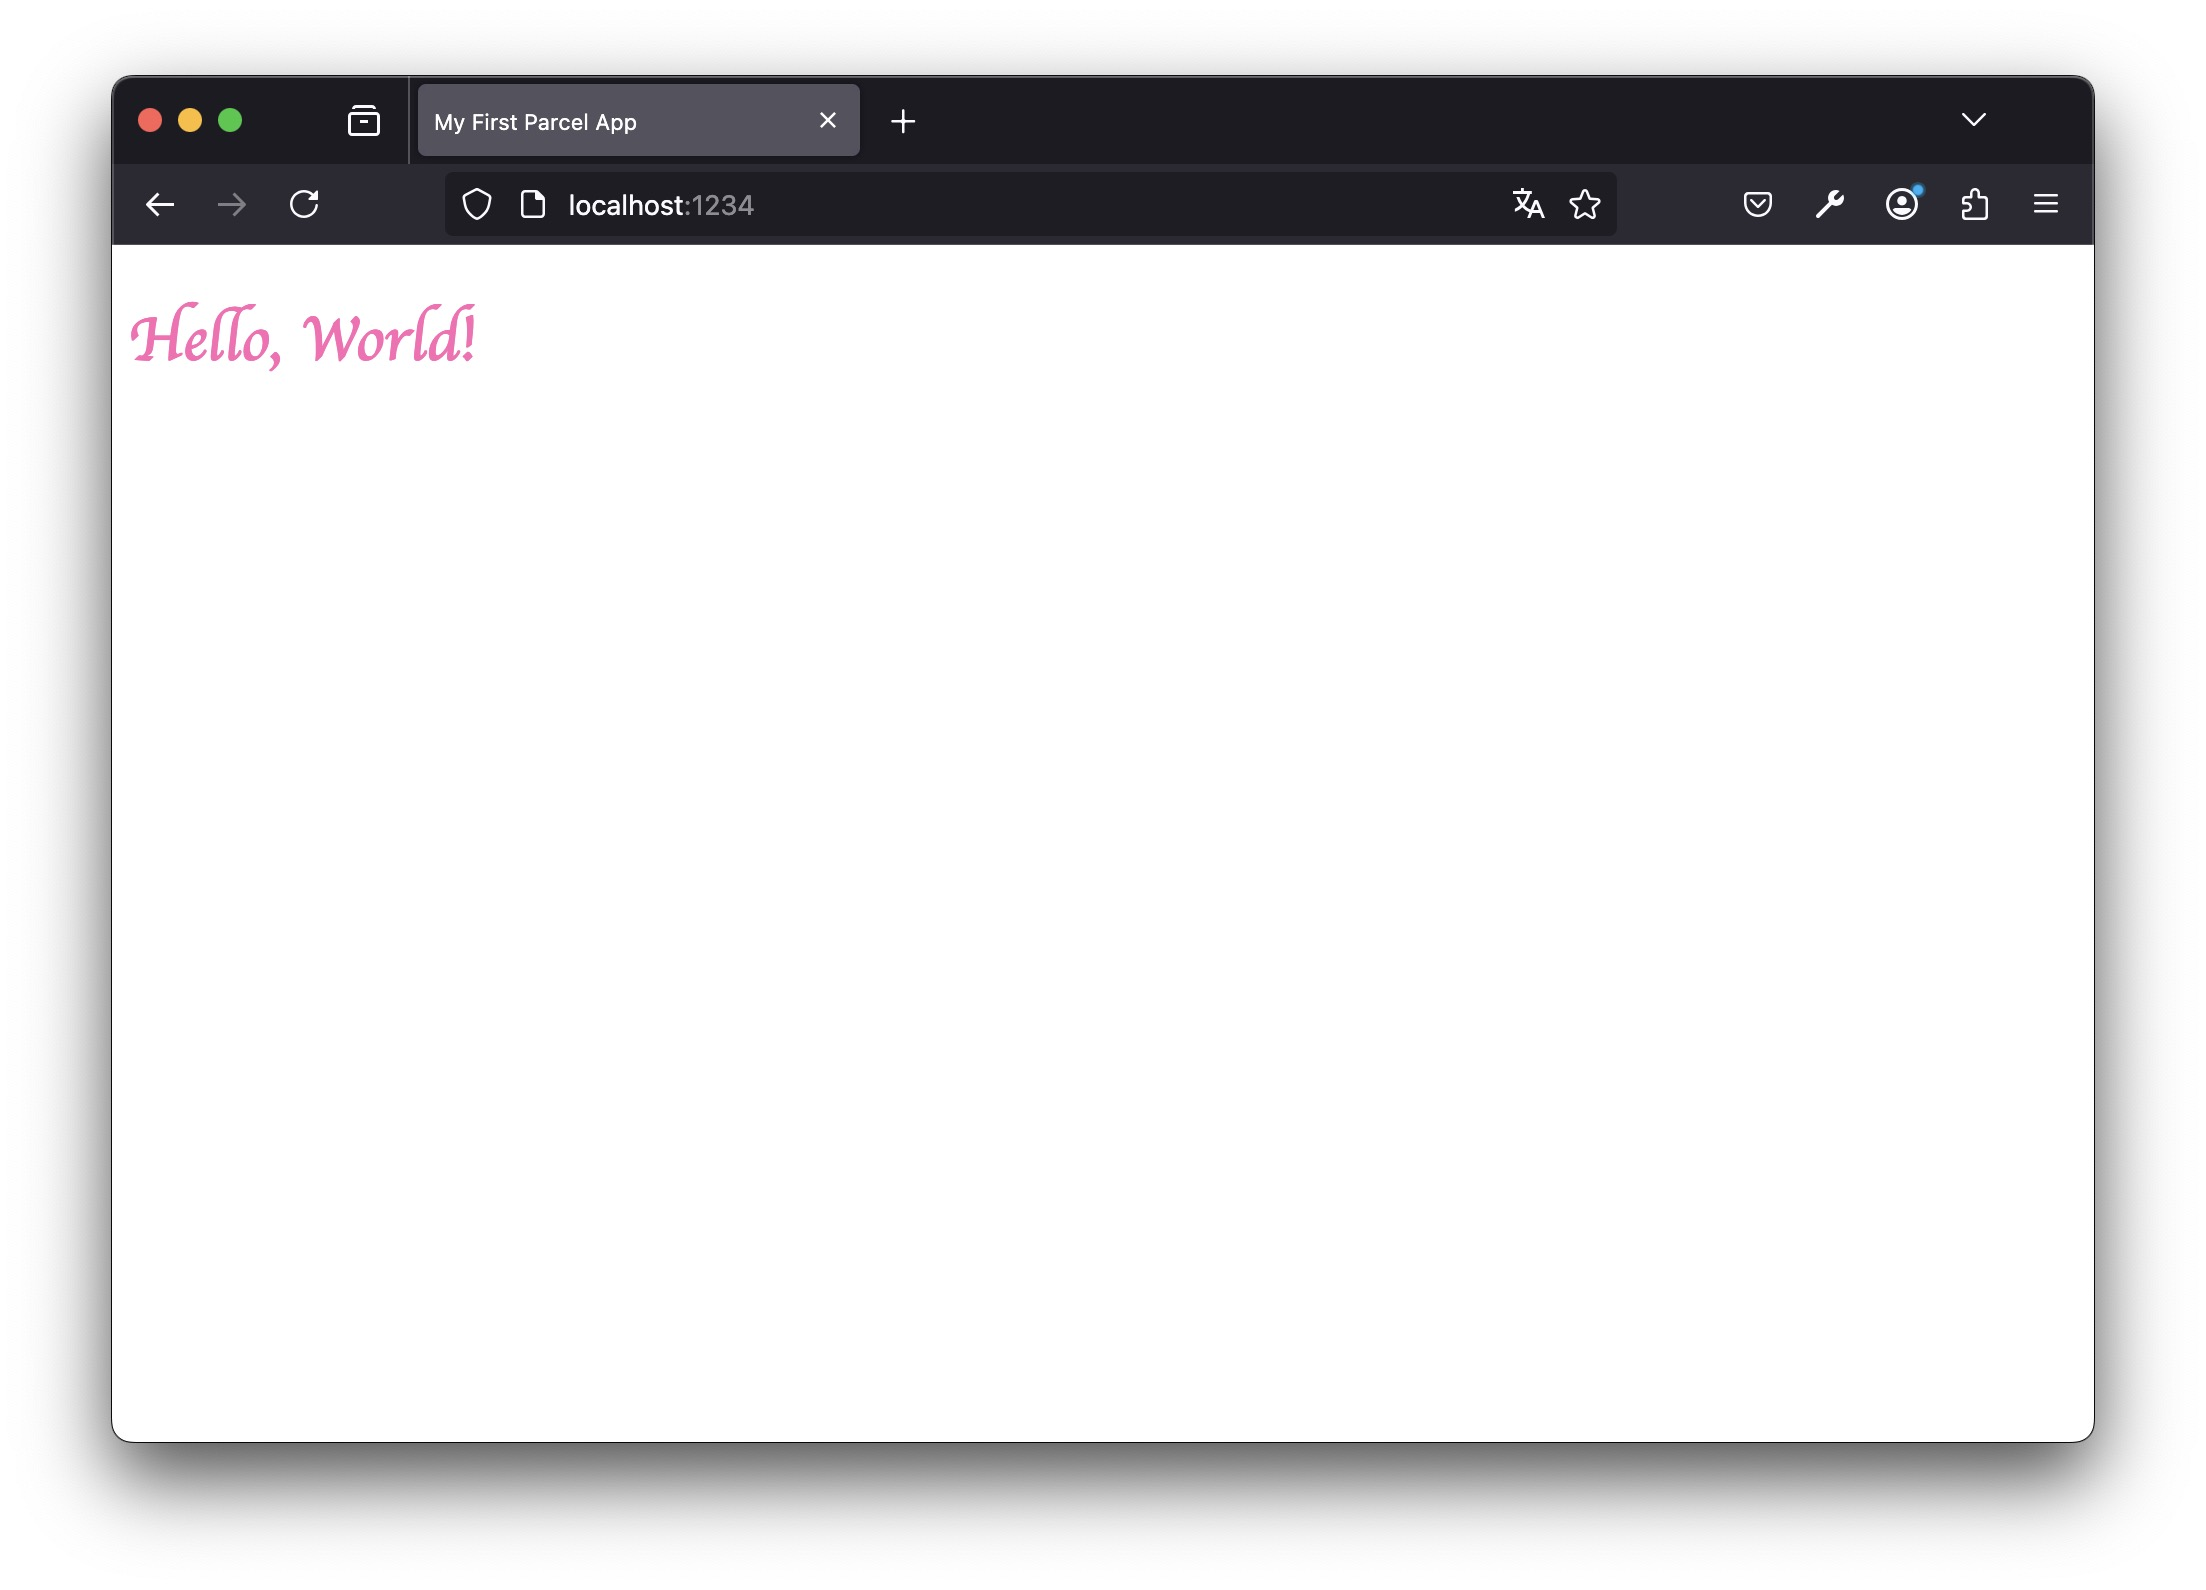
\includegraphics[width=0.8\textwidth]{./img/p1/hello-world-styled}
     \caption{Captura de pantalla de la página web con Parcel}
     \label{fig:parcel}
 \end{figure}

Por último, siguiendo el enunciado del Módulo 2, se ajustaron los scripts del \mintinline{bash}{package.json} para facilitar la ejecución de tareas comunes. Ahora, comandos como \mintinline{bash}{npm run start} y \mintinline{bash}{npm run build} simplifican el inicio del servidor de desarrollo y la compilación para producción, respectivamente. Además, se añadieron scripts para limpiar los directorios de caché y producción antes de cada compilación, como se muestra en la Figura~\ref{fig:package-json}.

\begin{figure}[h!]
\begin{minted}{json}
{
  "name": "hhyc-dramosac",
  "source": "src/index.html",
  "scripts": {
    "parcel:dev": "parcel",
    "parcel:build": "parcel build",
    "clean": "rimraf dist .parcel-cache",
    "start": "npm-run-all clean parcel:dev",
    "build": "npm-run-all clean parcel:build",
    "build:docs": "tectonic -Z shell-escape docs/p1.tex"
  },
  "author": "Daniel Ramos Acosta",
  "license": "ISC",
  "devDependencies": {
    "npm-run-all": "^4.1.5",
    "parcel": "^2.13.3",
    "rimraf": "^6.0.1"
  }
}
\end{minted}
\caption{Versión final del \lstinline{package.json}}
\label{fig:package-json}
\end{figure}

\subsection{Configuración de Pre y Post Procesadores}\label{subsec:configuracion-de-pre-y-post-procesadores}

El siguiente paso fue ajustar la configuración de \mintinline{bash}{browserslist} para garantizar la compatibilidad con navegadores desde 2011. Aunque esta configuración puede ser demasiado amplia, permitió comprobar que Parcel realiza las transformaciones necesarias para soportar navegadores antiguos. Esto asegura que la web sea accesible para una mayor audiencia.

Se ha comprobado que funciona correctamente. Parcel ha generado dos bundles de JavaScript, uno pensado para navegadores recientes que tengan soporte de módulos de EcmaScript 2015, y otro bundle para navegadores antiguos que no soporten módulos. Ambos scripts están referenciados desde el \mintinline{bash}{index.html}, y se cargan automáticamente en función de las capacidades del navegador (ver Figura~\ref{fig:index-html}).

\begin{figure}[h!]
\begin{minted}{html}
<!doctype html>
<html lang="en">
<head>
    <meta charset="utf-8">
    <title>My First Parcel App</title>
    <link rel="stylesheet" href="/index.4c105ba5.css">
    <script type="module" src="/index.9f6a43db.js"></script>
    <script src="/index.4ab9977a.js" nomodule defer></script>
</head>
<body><h1>Hello UOC!</h1></body>
</html>
\end{minted}
\caption{Hoja de estilos que incluye propiedades CSS que necesitarán prefijos}
\label{fig:index-html}
\end{figure}

Para comprobar el correcto funcionamiento de PostCSS, se modificó la hoja de estilos para incluir reglas que requieren prefijos para navegadores antiguos. Al construir la aplicación con Parcel, el fichero CSS resultante contenía los prefijos necesarios, como se muestra en la Figura~\ref{fig:styles-css}. Esto demuestra la utilidad de PostCSS para mantener la compatibilidad sin sacrificar la legibilidad del código.

\begin{figure}[h!]
\begin{minted}{css}
body {
  height: 100vh;
  color: #1f1f1f;
  background: linear-gradient(to bottom, #bada55, #c0ffee);
}

img {
  user-select: none;
}
\end{minted}
\caption{Hoja de estilos que incluye propiedades CSS que necesitarán prefijos}
\label{fig:styles-css}
\end{figure}

Por último, se ha instalado y configurado el plugin \mintinline{bash}{PostHTML Include}, que permite incluir fragmentos de HTML en otros ficheros HTML. De nuevo, para comprobar su correcto funcionamiento, se ha creado un componente de botón en un fichero HTML separado, y se ha incluido en el \mintinline{bash}{index.html} principal. Una vez se ha construido la aplicación con Parcel, el botón se ha renderizado correctamente en la página web (ver Figura~\ref{fig:posthtml-include}).

\begin{figure}[h!]
    \centering
    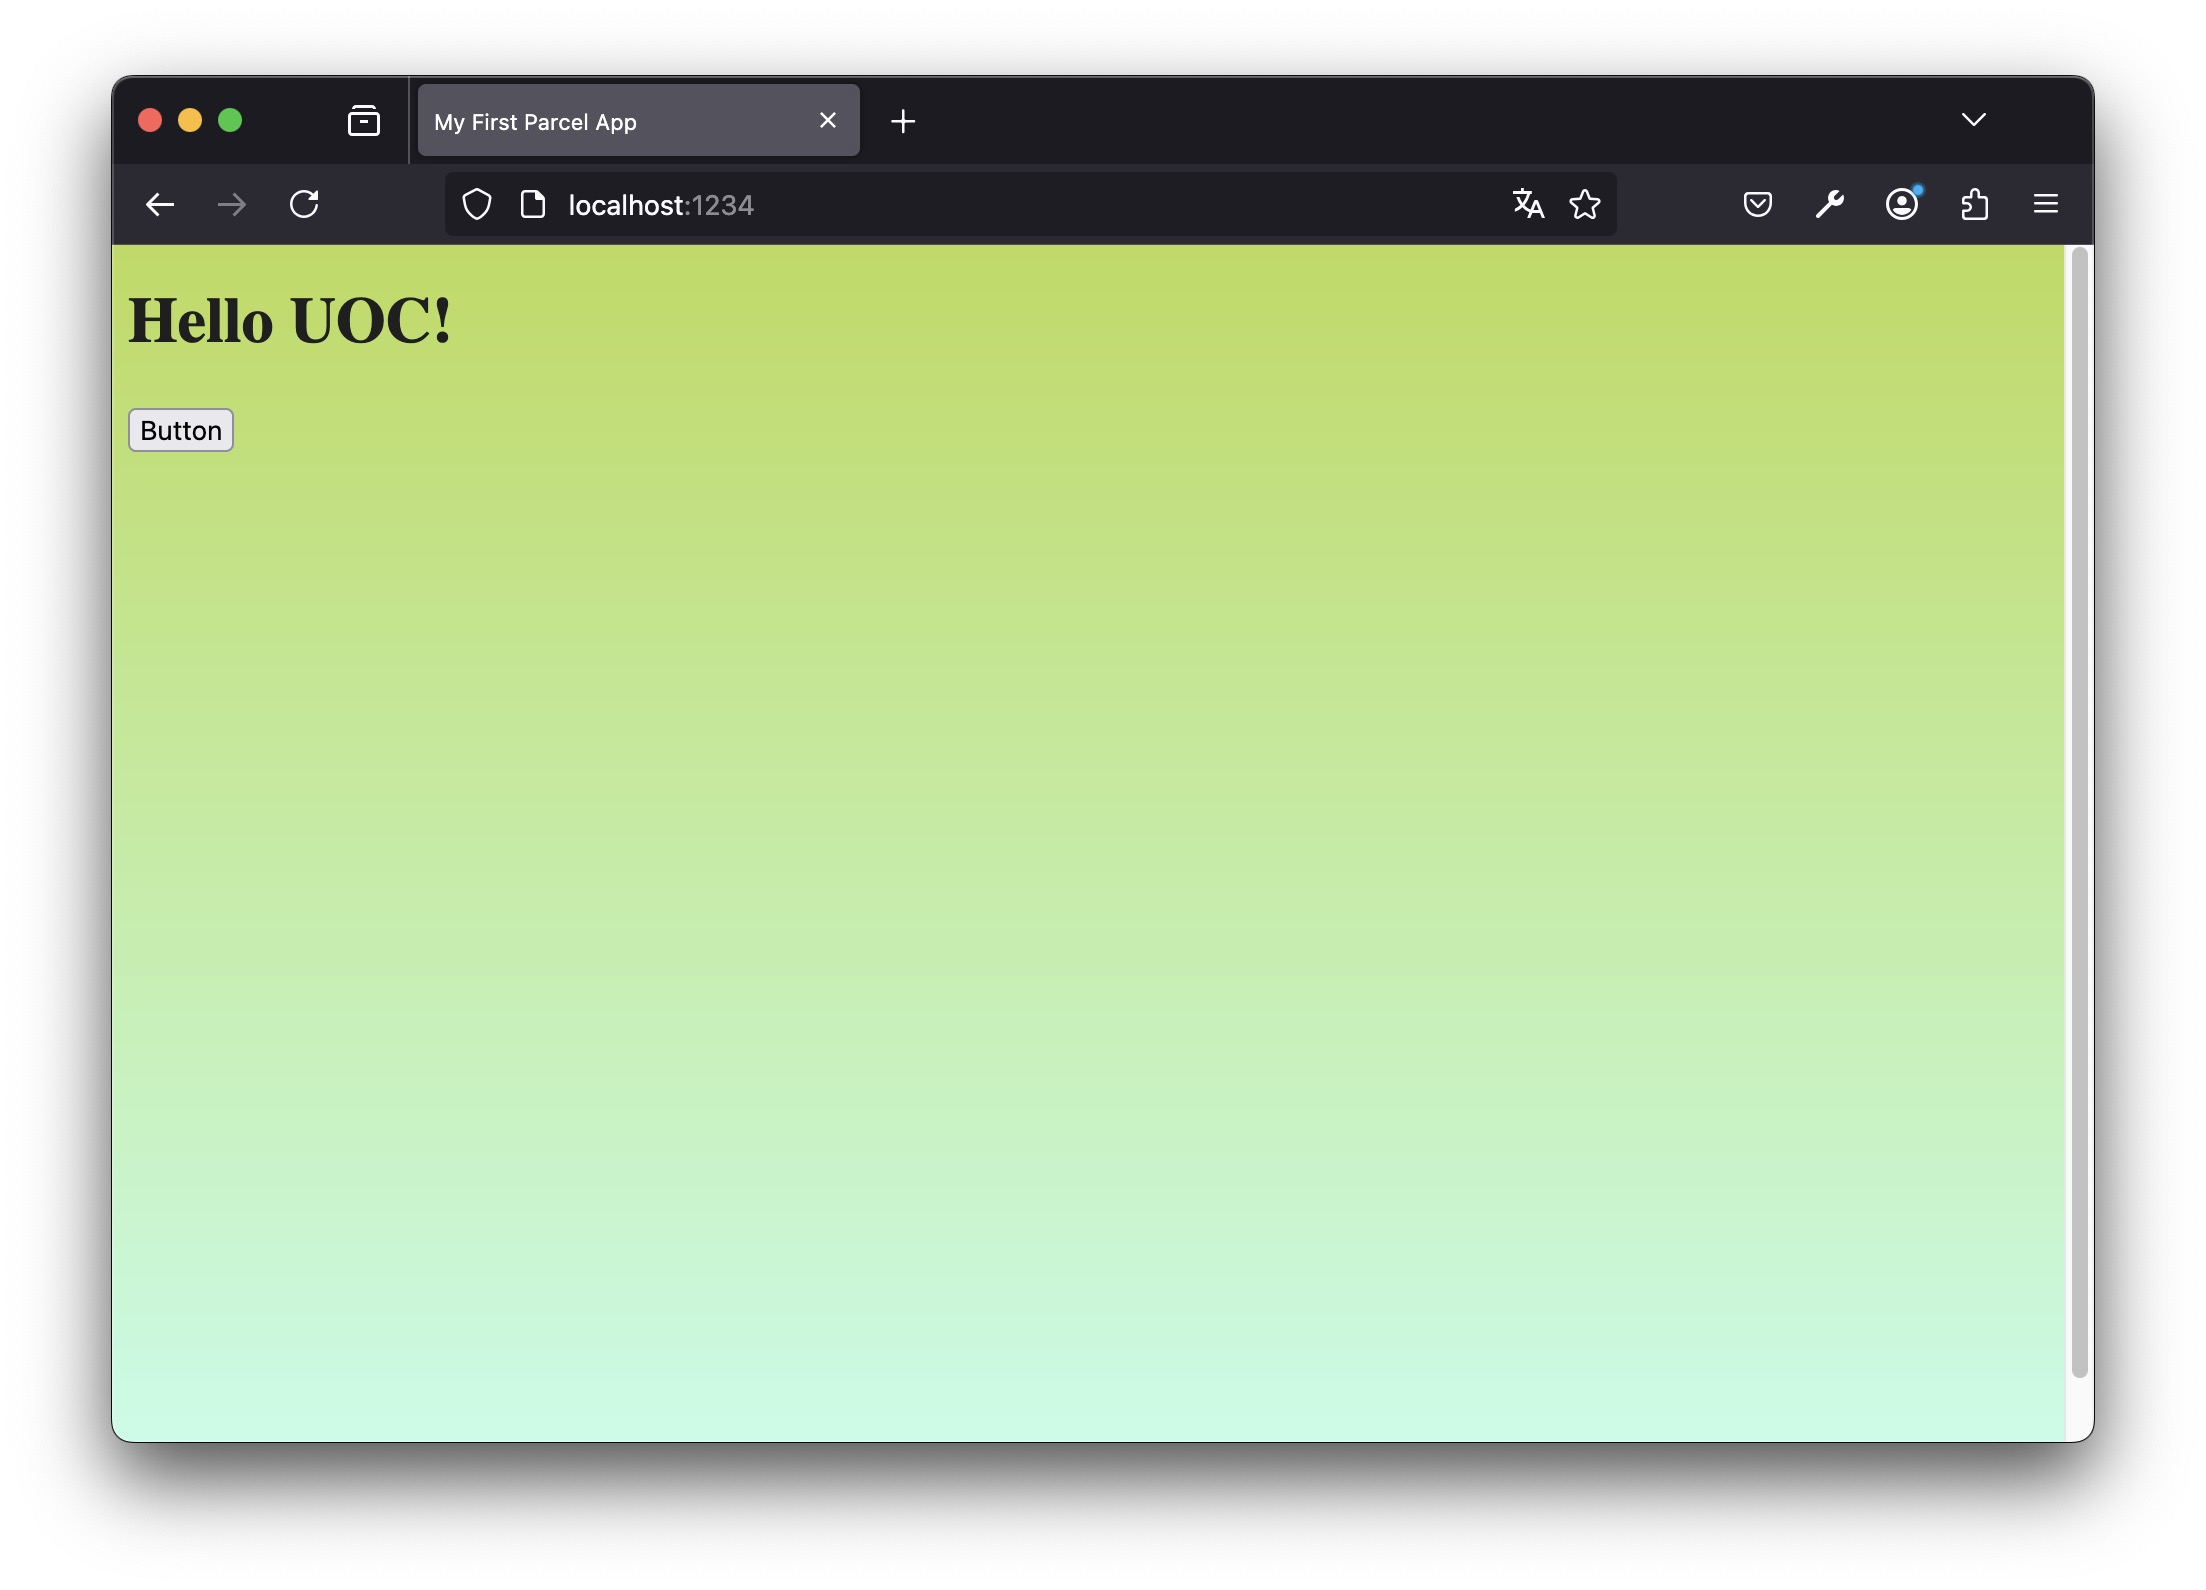
\includegraphics[width=0.8\textwidth]{./img/p1/after-posthtml-include}
    \caption{Captura de pantalla del navegador con el botón renderizado correctamente}
    \label{fig:posthtml-include}
\end{figure}

\subsection{Configuración del Despliegue}\label{subsec:configuracion-del-despliegue}

El despliegue automático de la web se configuró utilizando Github Pages, un servicio gratuito que permite publicar páginas web estáticas directamente desde un repositorio. Esto simplifica enormemente el proceso de publicación y asegura que la web esté siempre actualizada.

El siguiente paso ha sido configurar el despliegue automático de la web. En mi caso, he optado por usar Github Pages. Github Pages es un servicio gratuito de alojamiento web que ofrece Github, y que permite publicar páginas web estáticas directamente desde un repositorio de Github. Es una herramienta que he usado con anterioridad, y que resulta muy cómoda y fácil de configurar. En el caso de este proyecto, debemos configurar Github Pages para que publique usando Github Actions, ya que el proyecto requiere pasos previos de construcción. Para configurar el \textit{workflow}, he seguido la documentación oficial de la \textit{Action} \mintinline{bash}{upload-pages-artifact}, que proporciona un flujo de trabajo preconfigurado para publicar en Github Pages. En mi primer intento, la página web logró construirse correctamente, pero no llegó a publicarse ya que el \textit{workflow} falló en el paso de despliegue como se muestra en la Figura~\ref{fig:workflow-fail}.

\begin{figure}[h!]
    \centering
    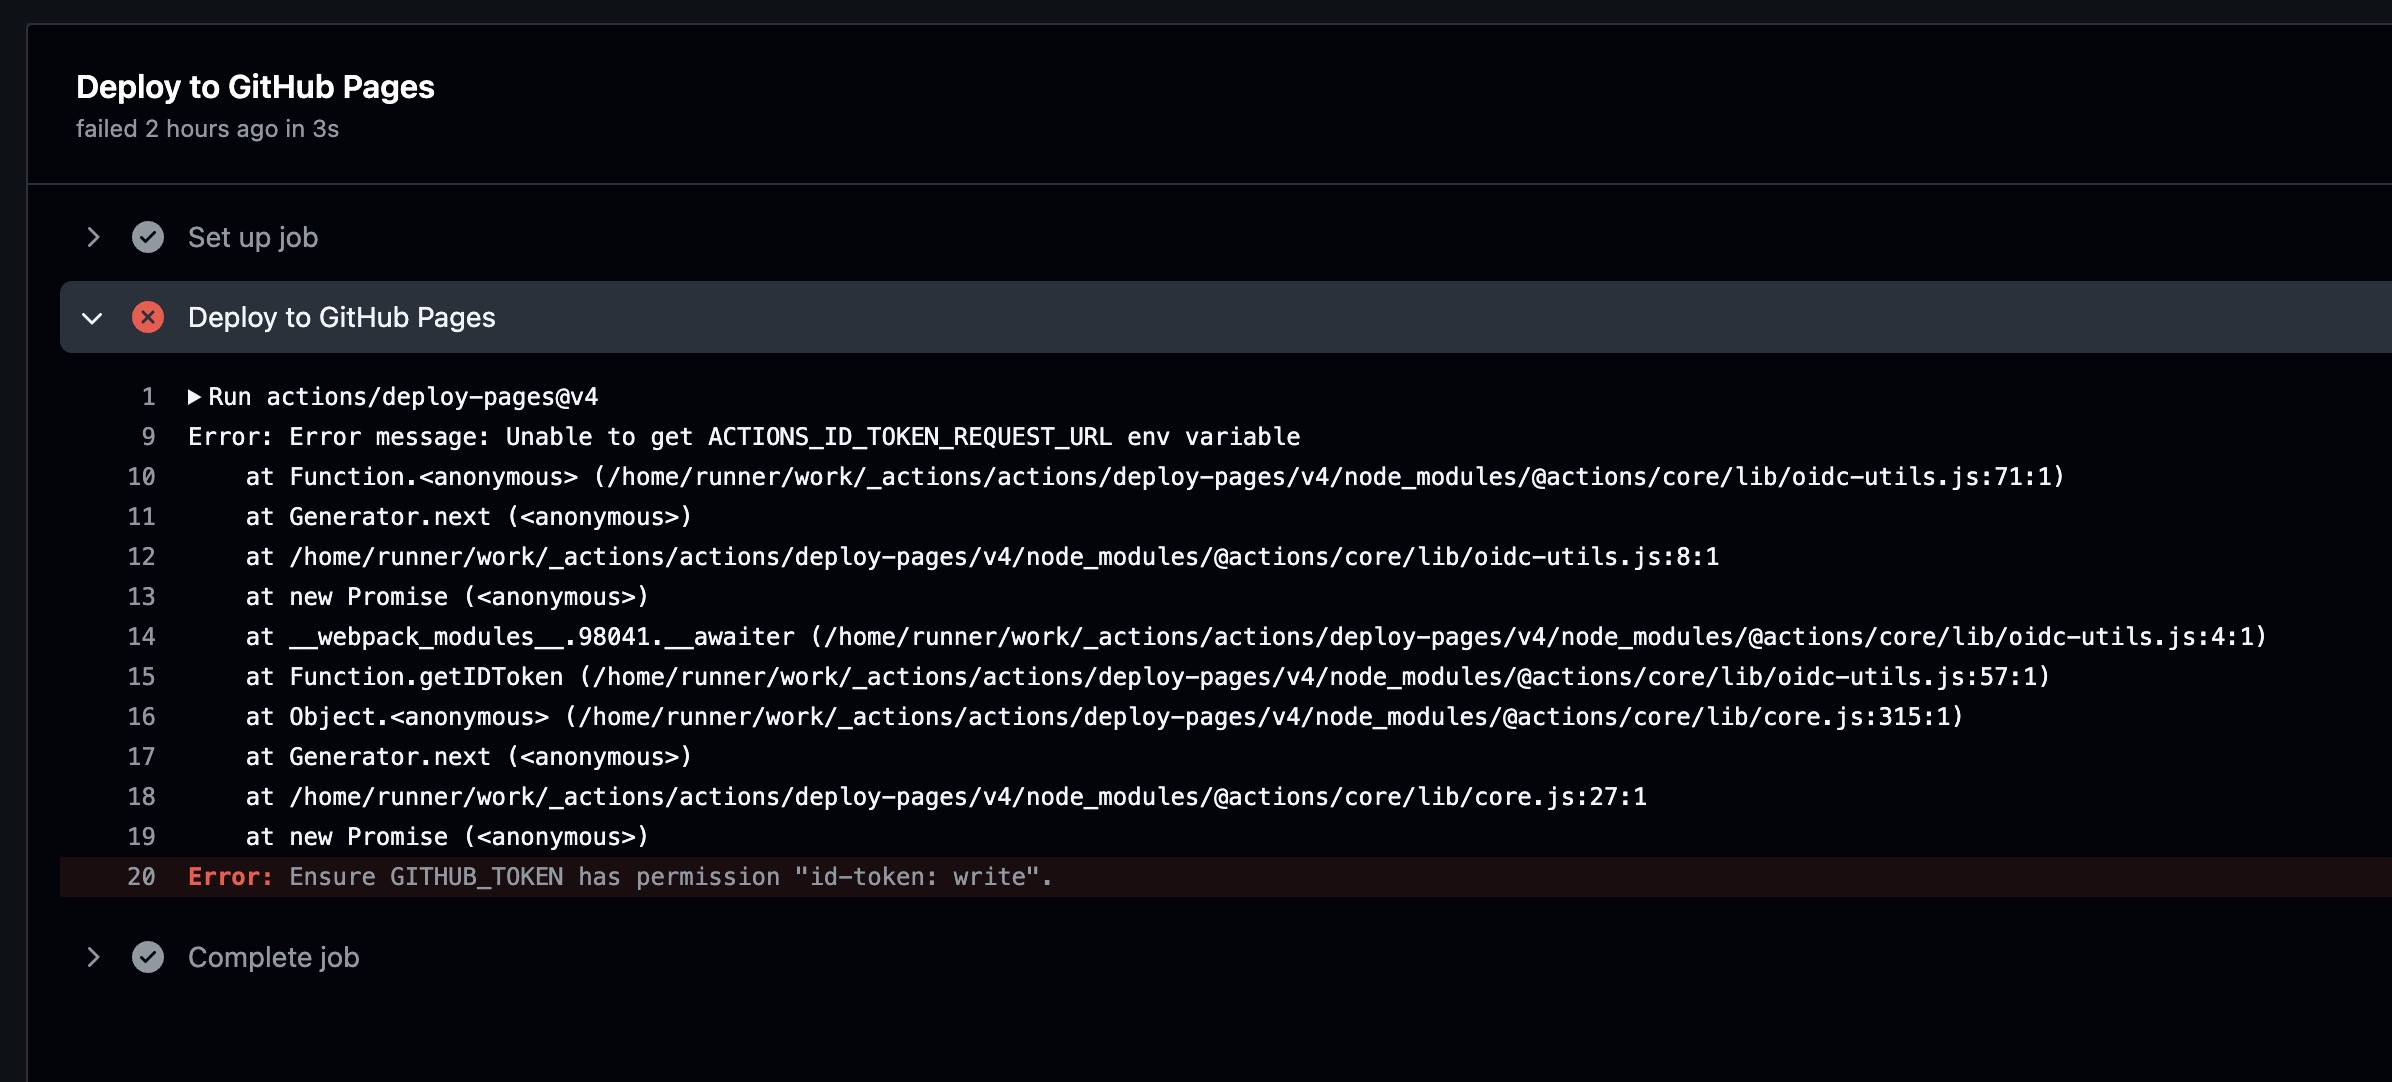
\includegraphics[width=0.8\textwidth]{./img/p1/workflow-failed}
    \caption{Captura de pantalla del fallo en el \textit{workflow} de despliegue}
    \label{fig:workflow-fail}
\end{figure}

Este fallo es un poco críptico, pero gracias a una respuesta de Stack Overflow (\href{https://stackoverflow.com/a/74167257}{enlace}), he podido identificar el problema. El problema es que el \textit{workflow} no tenía permisos para realizar la publicación, ya que es una acción de escritura.

La solución ha consistido en otorgar los permisos de configuración y escritura a la \textit{Action} de Github Pages. El \textit{workflow} se puede ver en la Figura~\ref{fig:workflow}.

\begin{figure}[h!]
\begin{minted}{yaml}
name: CI
permissions:
  contents: read
  pages: write
  id-token: write
on:
  push:
    branches:
      - main
jobs:
  website:
    name: Build Website
    runs-on: ubuntu-latest
    steps:
      - uses: actions/checkout@v4
      - uses: actions/setup-node@v4
        with:
          node-version: 'current'
      - run: npm install
      - run: npm run build
      - id: deployment
        uses: actions/upload-pages-artifact@v3
        with:
          path: ./dist
  deploy:
    name: Deploy to GitHub Pages
    environment:
      name: github-pages
      url: ${{ steps.deployment.outputs.page_url }}
    runs-on: ubuntu-latest
    needs: website
    steps:
      - id: deployment
        uses: actions/deploy-pages@v4
\end{minted}
\caption{Código de del \textit{workflow} para construir y desplegar la web}
\label{fig:workflow}
\end{figure}

La \textit{Action} lo que hace es:

\begin{enumerate}
    \item Clonar el repositorio
    \item Configurar la última versión LTS de Node.js
    \item Instalar las dependencias
    \item Construir la aplicación
    \item Subir los archivos estáticos como un artefacto
\end{enumerate}

Luego, la \textit{Action} de despliegue se encarga de publicar los archivos en Github Pages.

En cuanto se configuró correctamente, la página web logró verse en la URL \href{https://www.danielramos.me/hhyc-dramosac}, pero no se visualizaba correctamente ya que no cargaba la hoja de estilos como se puede ver en la Figura~\ref{fig:web-semi-deployed}.

\begin{figure}[h!]
    \centering
    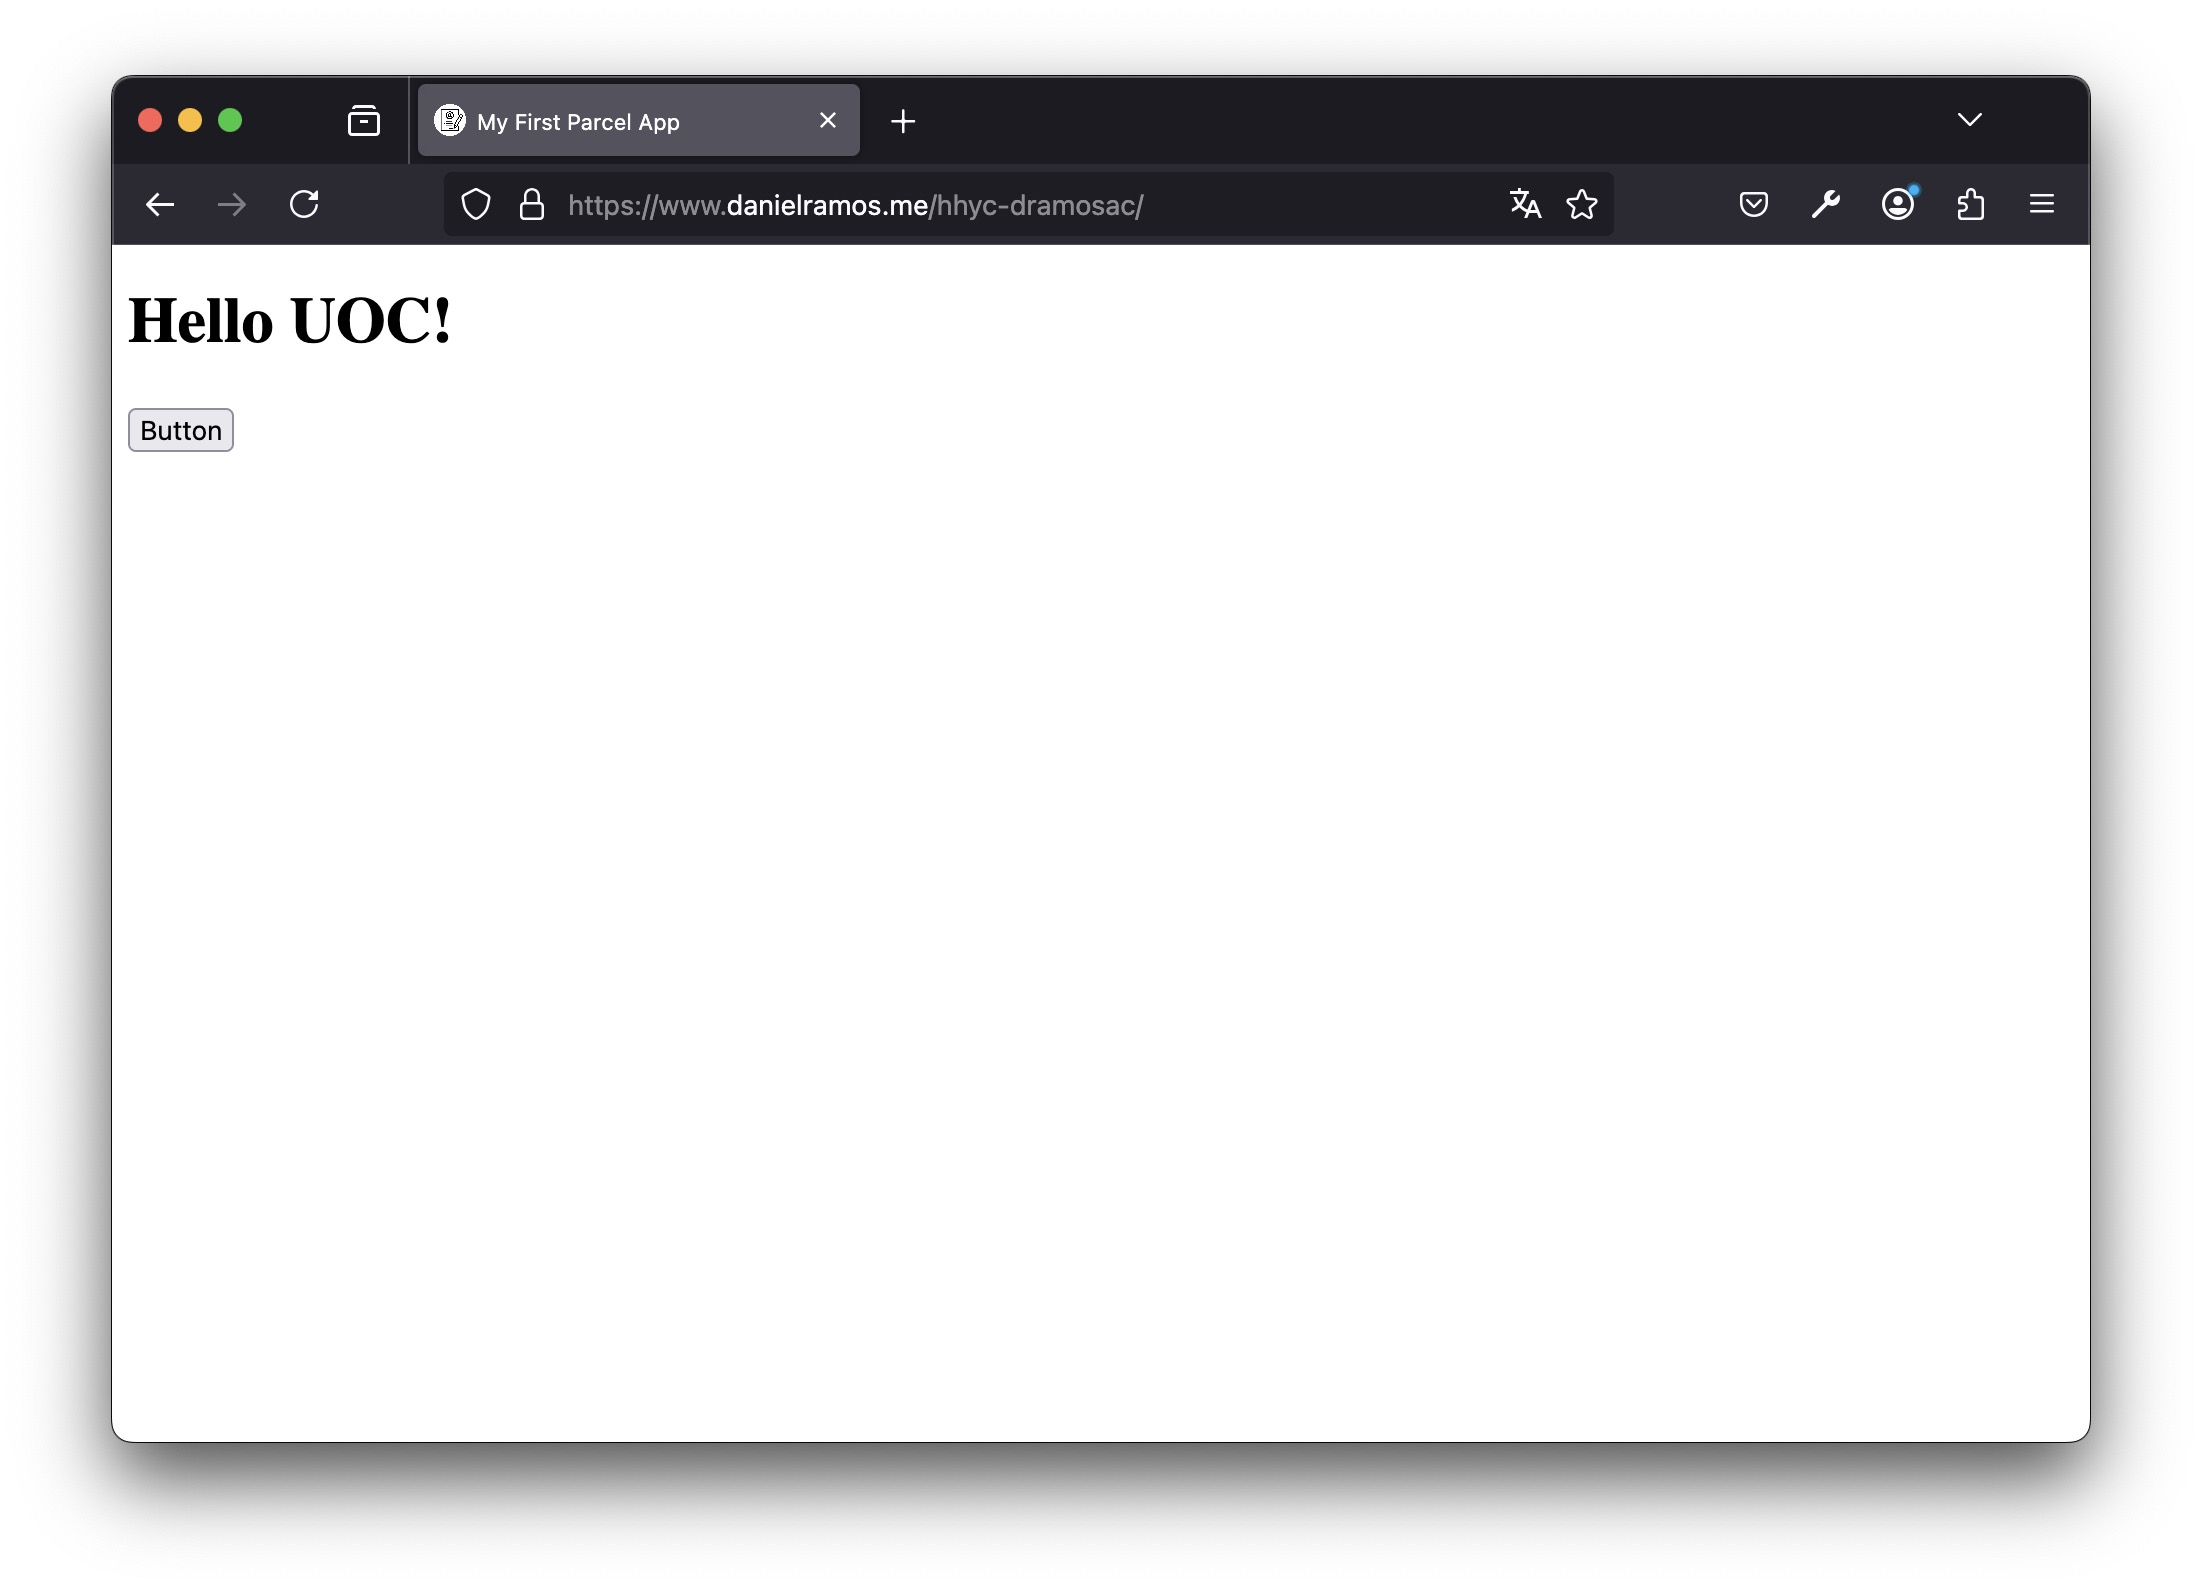
\includegraphics[width=0.8\textwidth]{./img/p1/web-semi-deployed}
    \caption{Captura de pantalla de la web desplegada en Github Pages, donde se aprecia que no se cargan los estilos}
    \label{fig:web-semi-deployed}
\end{figure}

Esto se debía a que la URL de la hoja de estilos, a pesar de que en local funcionaba, correctamente, como al desplegarse en Github Pages se hace en un subdirectorio, la URL relativa no era correcta. Para ello, Parcel tiene una opción llamada \mintinline{bash}{--public-url} que permite especificar la URL base de los recursos estáticos. He configurado esta opción para que la URL base sea \mintinline{bash}{./}, lo que hace que los recursos se carguen correctamente en Github Pages como se puede ver en la Figura~\ref{fig:web-deployed}.

\begin{figure}[h!]
    \centering
    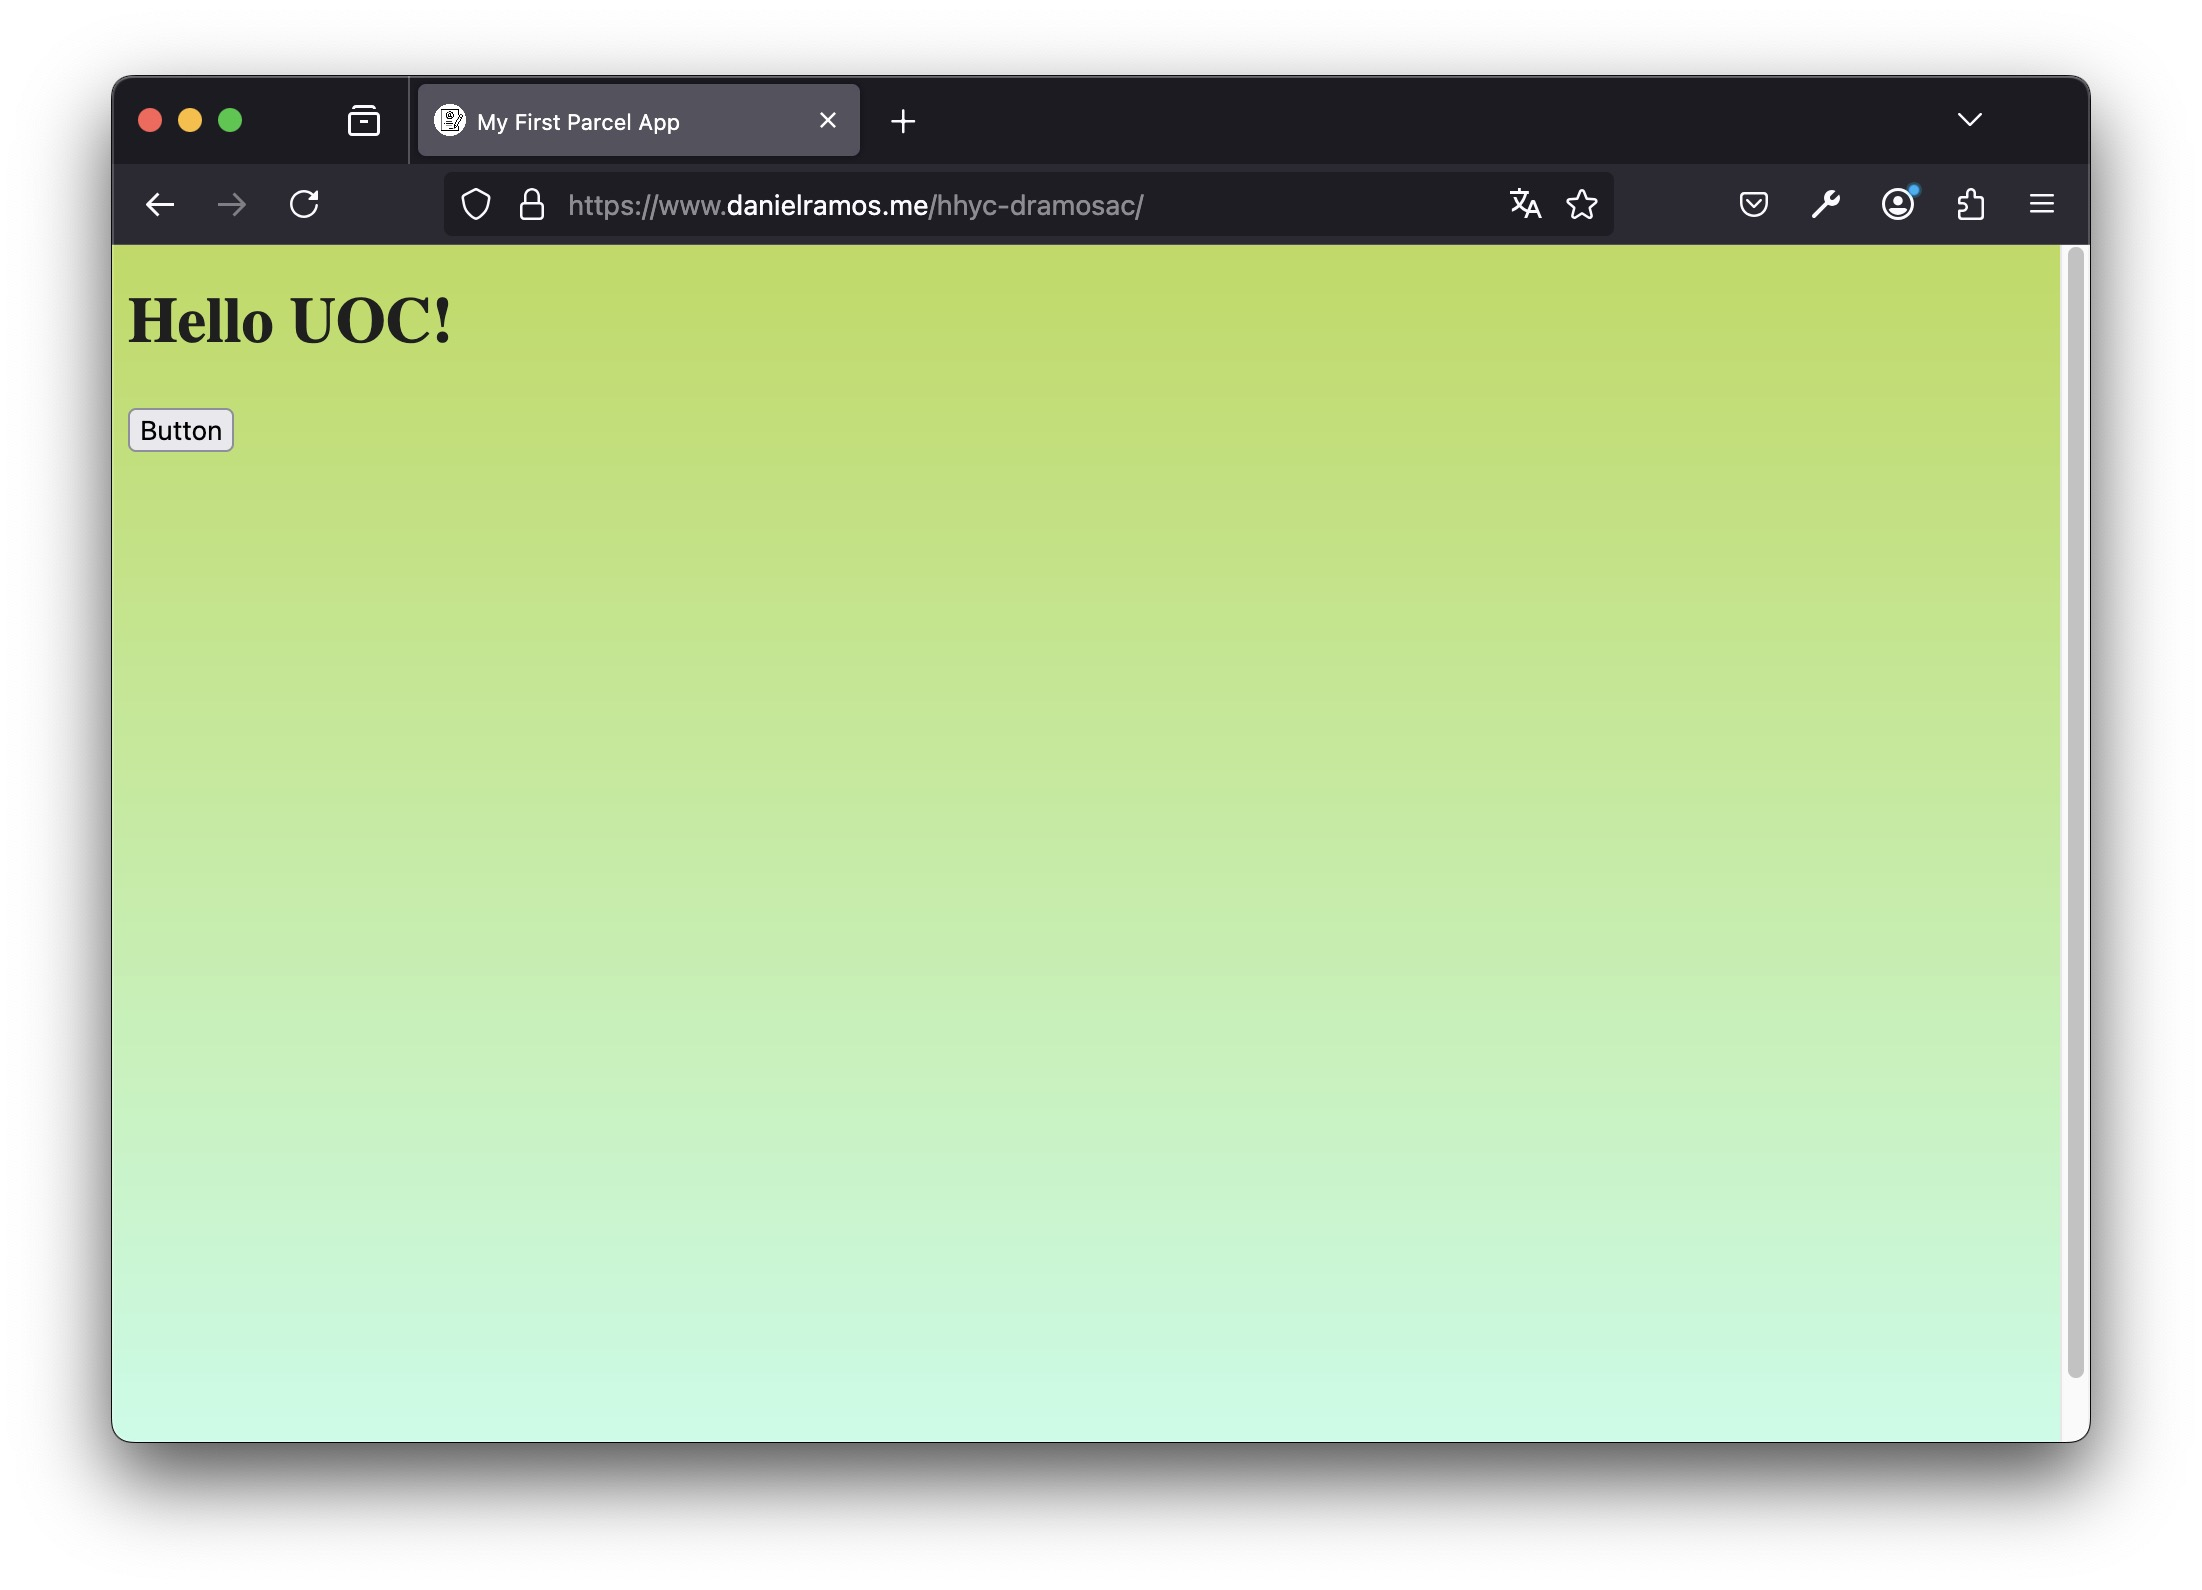
\includegraphics[width=0.8\textwidth]{./img/p1/web-deployed}
    \caption{Captura de pantalla de la web desplegada en Github Pages, donde ahora sí cargan los estilos}
    \label{fig:web-deployed}
\end{figure}

\subsection{Uso de GitHub Actions para la Construcción de la Documentación}\label{subsec:uso-de-github-actions-para-la-construccion-de-la-documentacion}

He decidido crear la documentación de esta práctica usando \LaTeX, e intentar seguir de forma más exacta posible la documentación proporcionada en materia de buenas prácticas en la redacción de documentos técnicos. Este documento \LaTeX se puede construir desde local usando \textit{Tectonic}, un compilador de LaTeX basado en el lenguaje de programación Rust. Sin embargo, para facilitar la construcción de la documentación, he decidido usar Github Actions. Para llevar a cabo esta tarea, he usado la documentación proporcionada en el propio \mintinline{bash}{README.md} del repositorio de \textit{Tectonic} (\href{https://github.com/marketplace/actions/setup-tectonic}{enlace}). Después de configurar el \textit{workflow}, he podido construir la documentación automáticamente al hacer un \textit{push} al repositorio.

\section{Desarrollo de la Web}\label{sec:desarrollo-de-la-web}

El desarrollo de la web siguió una estructura recomendada, incluyendo una página principal (\textit{Landing Page}), un listado de recetas, dos páginas de detalle y una página de fuentes. Se priorizó el uso de HTML semántico y la accesibilidad, verificando la compatibilidad con lectores de pantalla y la navegación mediante teclado.

Para garantizar la accesibilidad, se implementaron las siguientes prácticas:

\begin{itemize}
    \item Uso de etiquetas HTML semánticas como \texttt{<header>}, \texttt{<main>}, \texttt{<section>} y \texttt{<footer>} para estructurar el contenido de manera lógica y comprensible.
    \item Inclusión de atributos \texttt{alt} descriptivos en las imágenes necesarias para proporcionar contexto a los usuarios de lectores de pantalla.
    \item Implementación de etiquetas \texttt{aria-label} para mejorar la descripción de elementos interactivos como los enlaces de la paginación.
    \item Comprobar el correcto funcionamiento de la web con un lector de pantalla (ChromeBox Screen Reader), asegurando que el contenido se lee de manera coherente y comprensible.
\end{itemize}

Estas medidas aseguran que la web sea inclusiva y accesible para una amplia variedad de usuarios, incluyendo aquellos con discapacidades visuales, motoras o cognitivas.

\subsection{Uso de Procesadores}\label{subsec:uso-de-procesadores}

En esta práctica se ha hecho uso intensivo de la librería \mintinline{bash}{HTML Include}, que permite incluir fragmentos de HTML en otros ficheros HTML. Se ha seguido una estrategia de desarrollo basada en componentes, donde cada componente se ha desarrollado en un fichero HTML separado, y luego se han incluido en el \mintinline{bash}{index.html} principal.

Además, se ha incluido la librería \mintinline{bash}{postcss-nesting}, que permite usar la sintaxis de anidación de CSS en PostCSS. Esto es muy interesante, porque es una especificación que ya está soportada en navegadores modernos, pero que no está soportada en navegadores antiguos. Esto permite escribir CSS más limpio y legible, y Parcel se encarga de transformar el código para que sea compatible con navegadores antiguos.

\subsection{Dependencias Externas}\label{subsec:dependencias-externas}

Además de las herramientas mencionadas, se utilizó la librería \textit{Scroll Reveal} para implementar animaciones atractivas al hacer scroll. Esto mejoró significativamente la experiencia del usuario, haciendo la web más dinámica y visualmente atractiva.

\section{Conclusiones}\label{sec:conclusiones}

En esta práctica, se adquirieron habilidades clave para configurar un entorno de desarrollo moderno y eficiente. Parcel demostró ser una herramienta poderosa para gestionar recursos y automatizar tareas comunes. La integración con Github Actions y Pages permitió automatizar el despliegue y la construcción de la documentación, reduciendo errores y mejorando la productividad.

Además, el uso de librerías como \textit{Scroll Reveal} y \mintinline{bash}{postcss-nesting} permitió implementar características avanzadas y mantener un código limpio y compatible. En conjunto, esta práctica fue una experiencia enriquecedora que consolidó conocimientos y habilidades esenciales para el desarrollo web moderno.

\end{document}
